\documentclass[tikz,border=2pt]{standalone}
\usepackage{amsmath}
\usepackage{pgfplots}
\pgfplotsset{compat=1.18}
\usetikzlibrary{arrows.meta}
\begin{document}
% Fitted exponential density with rate 2/150: exact losses 20 and 30 contribute the density
% heights f(20), f(30); the loss capped at c = 100 contributes the tail area bar F(100) = e^{-4/3}.
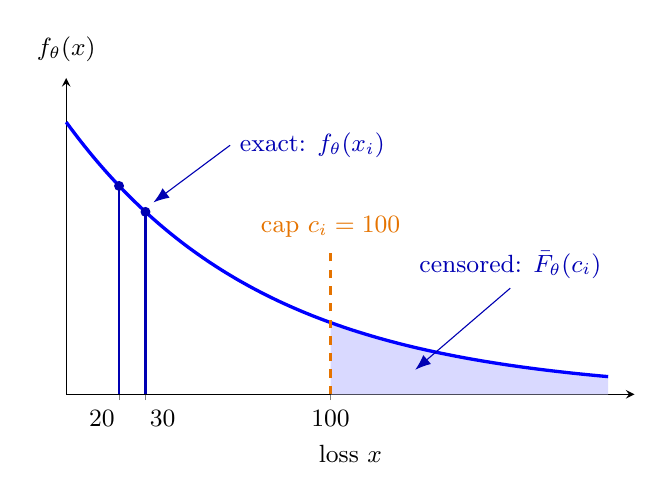
\begin{tikzpicture}[font=\small, >={Latex[length=2mm]}]
  \begin{axis}[
    axis lines=left, xmin=0, xmax=215, ymin=0, ymax=0.0155,
    xtick={20,30,100}, xticklabels={\makebox[0pt][r]{$20$\,},\makebox[0pt][l]{\,$30$},$100$}, ytick=\empty,
    xlabel={loss $x$}, ylabel={$f_\theta(x)$},
    ylabel style={rotate=-90, anchor=south, at={(axis description cs:0,1.02)}},
    samples=120, width=8.8cm, height=5.6cm, clip=false]
    \addplot[fill=blue!15, draw=none, domain=100:205] {(2/150)*exp(-2*x/150)} \closedcycle;
    \addplot[blue, very thick, domain=0:205] {(2/150)*exp(-2*x/150)};
    % exact observations: density heights
    \draw[blue!70!black, thick] (axis cs:20,0) -- (axis cs:20,0.010209);
    \draw[blue!70!black, thick] (axis cs:30,0) -- (axis cs:30,0.008937);
    \fill[blue!70!black] (axis cs:20,0.010209) circle (1.8pt);
    \fill[blue!70!black] (axis cs:30,0.008937) circle (1.8pt);
    \draw[blue!70!black, ->] (axis cs:62,0.0122) -- (axis cs:33,0.0094);
    \node[blue!70!black, anchor=west] at (axis cs:62,0.0122) {exact: $f_\theta(x_i)$};
    % censoring cap
    \draw[orange!90!black, thick, dashed] (axis cs:100,0) -- (axis cs:100,0.0072);
    \node[orange!90!black, anchor=south] at (axis cs:100,0.0072) {cap $c_i=100$};
    \draw[blue!70!black, ->] (axis cs:168,0.0052) -- (axis cs:132,0.0012);
    \node[blue!70!black, anchor=south] at (axis cs:168,0.0052) {censored: $\bar F_\theta(c_i)$};
  \end{axis}
\end{tikzpicture}
\end{document}
